%
% Copyright (c) 2022 Antonio Coín Castro
%
% This work is licensed under a
% Creative Commons Attribution-ShareAlike 4.0 International License.
%
% You should have received a copy of the license along with this
% work. If not, see <http://creativecommons.org/licenses/by-sa/4.0/>.
%

\RequirePackage{fix-cm}
\documentclass[9pt, english, professionalfonts]{beamer}

% PACKAGES

\usepackage{fontspec}
\usepackage[autostyle=true]{csquotes}
\usepackage[absolute,overlay]{textpos}
\usepackage[english]{babel}
\usepackage{microtype}
\usepackage{subcaption}
\usepackage{epigraph}
\usepackage[export]{adjustbox}
\usepackage{hyperref}
\usepackage{bm}
\usepackage{amssymb, amsmath, amsthm, amsfonts, amscd, dsfont}

% BEAMER OPTIONS

\usetheme[block=fill, subsectionpage=progressbar, titleformat section=smallcaps]{metropolis}
\setbeamertemplate{frametitle continuation}[roman]
\setbeamerfont{section title}{size=\huge}
\setbeamertemplate{section in toc}[sections numbered]
%\setbeamertemplate{subsection in toc}[subsections unnumbered]
\widowpenalties 1 10000
\raggedbottom

\renewcommand{\thefootnote}{\fnsymbol{footnote}}
\renewcommand{\baselinestretch}{1.3}

% COLORS

\definecolor{Maroon}{cmyk}{0, 0.87, 0.88, 0.1}
\definecolor{teal}{rgb}{0.0, 0.45, 0.45}
\definecolor{mLightBrown}{HTML}{f97e0b}
% \definecolor{mLightBrown}{HTML}{990000}  % Darker accent color
% \definecolor{backg}{HTML}{F2F2F2} % Fondo
% \definecolor{comments}{HTML}{a8a8a8} % Comentarios
% \definecolor{keywords}{HTML}{08388c} % Palabras clave
% \definecolor{strings}{HTML}{0489B1}  % Strings
\setbeamercolor{palette primary}{bg=teal}
\setbeamercolor{progress bar}{use=Maroon, fg=Maroon}

% BIBLIOGRAPHY

\usepackage[backend=biber,style=numeric-comp,sorting=none]{biblatex}
\addbibresource{bibliography.bib}
\setbeamertemplate{bibliography item}[article]

% GRAPHICS

\graphicspath{%
  {../figures/}
}

% CUSTOM COMMANDS

\newcommand\maroon[1]{\color{mLightBrown}#1\color{mDarkTeal}}
\renewcommand{\epsilon}{\varepsilon}

%% Math operators
\DeclareMathOperator*\argmin{arg\,min}
\DeclareMathOperator\supp{supp}
\DeclareMathOperator\Cov{Cov}
\DeclareMathOperator\Var{Var}

%% Math symbols
\newcommand{\N} {\ensuremath{\mathds{N}}}
\newcommand{\R} {\ensuremath{\mathds{R}}}
\newcommand{\E} {\ensuremath{\mathds{E}}}
\newcommand{\I} {\ensuremath{\mathds{I}}}
\renewcommand{\P} {\ensuremath{\mathds{P}}}

\newcommand{\D} {\ensuremath{\mathcal{D}}}
\newcommand{\X} {\ensuremath{\mathcal{X}}}
\newcommand{\K} {\ensuremath{\mathcal{K}}}
\newcommand{\T} {\ensuremath{\mathcal{T}}}
\newcommand{\U} {\ensuremath{\mathcal{U}}}
\newcommand{\Lcal} {\ensuremath{\mathcal{L}}}
\newcommand{\Hcal} {\ensuremath\mathcal{H}}

%% Scalar product
\newcommand\dotprod[2]{\left\langle #1, #2 \right\rangle}

% TITLE

\title{\huge{Bayesian RKHS-based methods in functional regression}}
\providecommand{\subtitle}[1]{}
\subtitle{\Large{Master's degree in Data Science}}
\date{\normalsize{September 20th, 2022}\vspace{1em}\\\normalsize{Master's thesis}\vspace{2em}}
\author{\normalsize{Antonio Coín Castro}}
\institute{\small{Supervisors:\\José Ramón Berrendero Díaz\\ Antonio Cuevas González}}

\titlegraphic{
  \begin{textblock*}{2cm}(6.7cm, 7.5cm)
    
\includegraphics[width=5cm]{uam_eps_logo}
  \end{textblock*}
}

% DOCUMENT

\begin{document}
\maketitle

% \begin{frame}{Table of contents}
%    \tableofcontents
% \end{frame}

\section{Introduction}

\begin{frame}{What is FDA?}
\begin{center}
  \Large{\maroon{Functional Data Analysis}}
\end{center}
\vspace{1em}
\begin{figure}[ht!]
  \centering
  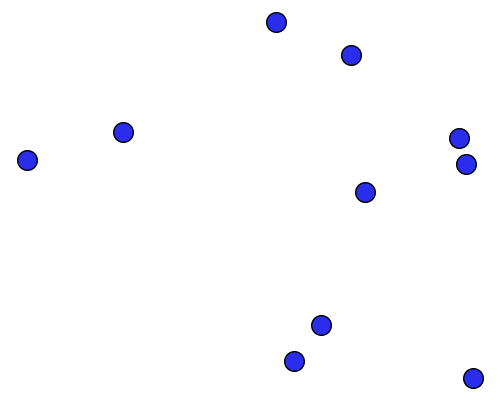
\includegraphics[width=.3\textwidth, valign=c]{example_points}
  \hspace{.4cm}
  \Huge{\(\longrightarrow\)}
  \hspace{.2cm}
  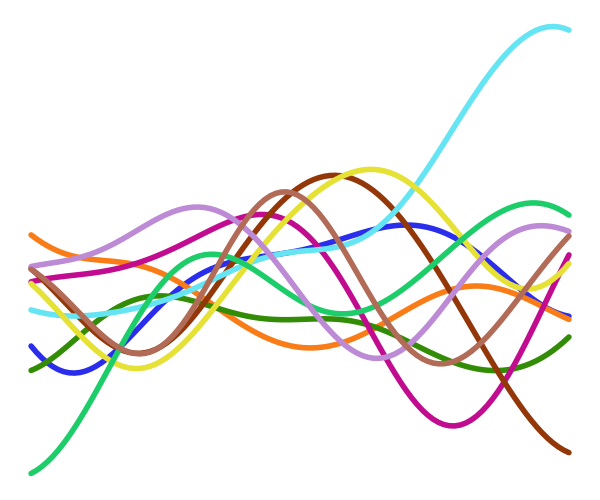
\includegraphics[width=.35\textwidth, valign=c]{example_functions}
  % Captions
  \large
  \makebox[.3\textwidth]{\(\R^p\)}
  \hspace{.4cm}
  \phantom{\(\longrightarrow\)}
  \hspace{.2cm}
  \makebox[.35\textwidth]{\(L^2[0,1]\)}
\end{figure}
\vspace{1em}
\normalsize
\begin{center}
\parbox{9cm}{\centering \textit{Statistical techniques to process, model and make inference on data varying over a continuum}}
\end{center}
\end{frame}

\begin{frame}{Functional linear regression}
  \maroon{First problem}: linear regression with functional data.
  \vspace{2em}

\begin{figure}
    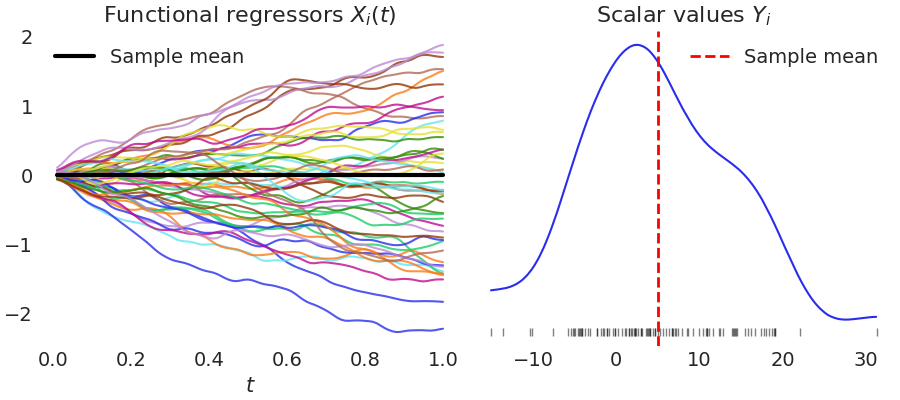
\includegraphics[width=\textwidth]{data_lin}
  \end{figure}
\end{frame}

\begin{frame}{Functional logistic regression}
  \maroon{Second problem}: logistic regression with functional data.
\vspace{2em}

\begin{figure}
    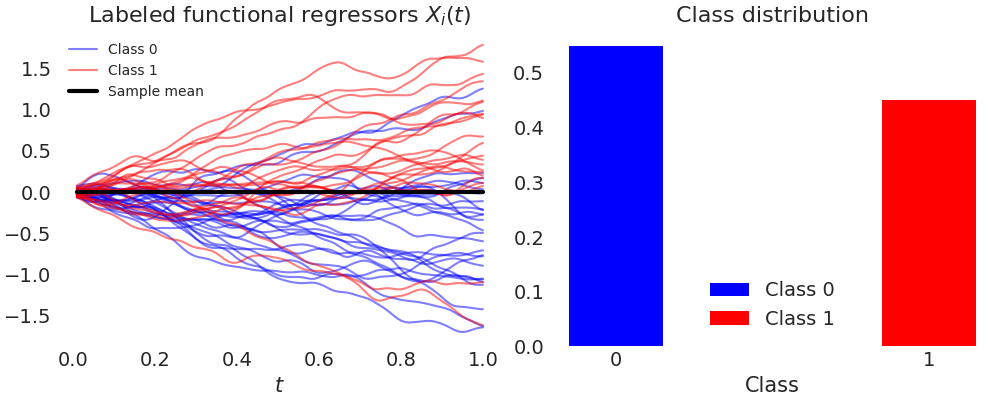
\includegraphics[width=\textwidth]{data_log}
  \end{figure}
\end{frame}

\begin{frame}{The usual \(\bm{L^2}\)-models}
  \(\bullet\) \(X=X(t)\) second order stochastic process with trajectories in \(L^2[0, 1]\).

  \(\bullet\) \(Y\) real variable (continuous or dichotomous).

  \vspace{1em}

\begin{block}{Linear \(\bm{L^2}\)-model}
  \[
    Y = \alpha_0 + \maroon{\langle X, \beta \rangle_2} + \varepsilon = \alpha_0 + \int_0^1 X(t)\beta(t)\, dt + \varepsilon.
  \]
\end{block}

\begin{block}{Logistic \(\bm{L^2}\)-model}
    \[
    \mathbb P (Y=1\mid X) = \frac{1}{1 + \exp\{-\alpha_0 - \maroon{\langle X, \beta\rangle_2}\}} = \frac{1}{1 + \exp\{-\alpha_0 - \int_0^1 X(t)\beta(t)\, dt\}}.
  \]
\end{block}
  \maroon{\(\beta \in L^2[0,1]\)}, \(\alpha_0\in\mathbb R\), \ \(\varepsilon \sim \mathcal N(0, \sigma^2), \ X \bot \varepsilon\).

  \footnotetext{\includegraphics[scale=.7]{beamericonbook} \ Ramsay, J. and Silverman, B. (1997). \textit{Functional Data Analysis}.}
\end{frame}

\begin{frame}{Shortcomings of the \(\bm{L^2}\)-models}
  \begin{itemize}
    \item Direct optimization is hopeless: \(L^2[0,1]\) is a \maroon{extremely wide space}.
    \item The usual least-squares theory cannot be applied directly; some regularization or dimensionality reduction techniques are required.
    \item They do not include simple models based on linear combinations of the marginal of the process as particular cases, such as
    \[
      Y = \alpha_0 + \sum_{j=1}^p \beta_j X(t_j) + \varepsilon.
    \]
    \item In the logistic case, the maximum likelihood estimator does not exist with probability 1 under fairly general conditions.
  \end{itemize}
\end{frame}

\section{A RKHS model for functional regression}


\begin{frame}{Alternative model: RKHS}

We will exploit the theory of \textit{reproducing kernel Hilbert spaces} (RKHS's).

\vspace{1em}
\begin{alertblock}{Proposal\footnote[2]{Based on the work of Berrendero et al. (2019) and Berrendero et al. (2022).}}
  Change the habitat of the functional parameter \(\beta(\cdot)\).
\end{alertblock}

\vspace{1em}
  We consider a functional parameter \maroon{\(\alpha \in \Hcal(K)\)}, where \(\Hcal(K)\) is the RKHS associated with the covariance function \(K(t, s)=\mathbb E[X(t)X(s)]\) of the centered process \(X\). Moreover, we substitute \(\dotprod{X}{\beta}_2\) for \maroon{\(\dotprod{X}{\alpha}_K\)}.
\end{frame}

\begin{frame}{Historical review of RKHS theory}
  \begin{itemize}
    \item Initial development \(\longrightarrow\) 1950's (Mercer, Aronszajn, Bergman).
    \item Uses in statistics \(\longrightarrow\) 1960's, 1970's (Parzen, Wahba, \ldots).
    \item Uses in Machine Learning \(\longrightarrow\) 1990's, 2000's (representer theorems).
    \item Uses in FDA \(\longrightarrow\) 2010's onwards.
  \end{itemize}
\end{frame}

\begin{frame}{RKHS's in a nutshell}
  \begin{definition}
    Start with the preliminary space
    \[
    \Hcal_0(K) = \left\{ f \in L^2[0,1]: \ f(\cdot) = \sum_{i=1}^p a_i K(t_i, \cdot), \ p \in \N,  a_i \in \R,  t_i \in [0, 1] \right\},
    \]
    which is endowed with the scalar product \(\dotprod{f}{g}_K = \sum_{i, j} a_i b_j K(t_i, s_j)\), for \(f(\cdot)=\sum_i a_i K(t_i, \cdot) \) and \(g(\cdot)=\sum_j b_j K(s_j, \cdot)\).

    Then, \(\Hcal(K)\) is the completion of \(\Hcal_0(K)\) under this scalar product.
  \end{definition}

  \vspace{1em}

  Note that \(\Hcal(K)\subset L^2[0, 1]\) as subsets, but the elements of \(\Hcal(K)\) are simpler and more manageable in general. Plus, it is a space of \maroon{functions}, and not of equivalence classes.
\end{frame}

\begin{frame}{RKHS's in a nutshell (cont.)}
  This space has some interesting properties:

  \vspace{1em}

  \begin{block}{Proposition}
    \begin{enumerate}
      \item All the evaluation operators \(\delta_t(f)=f(t)\) are continuous \maroon{(characterization)}.
      \item Norm convergence implies pointwise convergence.
      \item If \(K\) is continuous, then so is every function \(f\in\Hcal(K)\).
    \end{enumerate}
  \end{block}
\end{frame}

\begin{frame}{A small subtlety}

  Generally speaking, the concrete realizations \(x=X(\omega)\) \maroon{do not belong to \(\Hcal(K)\) with probability 1}, so the expression \(\dotprod{x}{\alpha}_K\) lacks meaning. However, we can make use of the relationship between \(\Hcal(K)\) and \(\Lcal(X)\), the linear span of the process \(X\) within \(L^2(\Omega)\).

  \vspace{1em}
  \begin{block}{Loève's isometry}
    It is the continuous extension of the correspondence
    \[
\sum_{j=1}^p a_j X(t_j) \longleftrightarrow \sum_{j=1}^p a_j K(t_j, \cdot).
    \]
    Formally, \(\Psi^{-1}_X(U)(t) := \E[U X(t)]\) for \(U \in \Lcal(X)\).
  \end{block}
  With a slight abuse of notation, we will write \maroon{\(\dotprod{x}{\alpha}_K \equiv [\Psi_X(\alpha)](\omega) := \Psi_x(\alpha)\)}\ for \(x=X(\omega)\) and \(\alpha \in \Hcal(K)\).
\end{frame}

\begin{frame}{A new functional parameter\ldots}
  \begin{itemize}
    \item The initial idea was to suppose \(\alpha \in \Hcal(K)\).
    \item To further simplify the model, we will assume \(\alpha \in \Hcal_0(K)\), which is dense in \(\Hcal(K)\) by construction. That is,
    \[
      \alpha(\cdot) = \sum_{j=1}^p \beta_j K(t_j, \cdot), \quad \beta_j \in \R, \ t_j \in [0, 1], \ p \in \N.
    \]
    \item When evaluating \(\dotprod{x}{\alpha}_K\) for a trajectory \(x=X(\omega)\), we resort to Loève's isometry:
    \[
      \dotprod{x}{\alpha}_K = \Psi_x(\alpha) = \sum_{j=1}^p \beta_j X(t_j).
    \]
  \end{itemize}

\end{frame}

\begin{frame}{\ldots and two new models}
  Given a data set \(\D_n = \{(X_i, Y_i): i=1,\dots, n\}\) composed of i.i.d. samples of \((X, Y)\), for \(\alpha \in \Hcal_0(K)\) we consider the following models:

  \vspace{1em}

  \begin{block}{Linear RKHS model}
  \[
    Y_i = \alpha_0 + \maroon{\langle X_i, \alpha \rangle_K} + \varepsilon = \alpha_0 + \sum_{j=1}^p \beta_j X_i(t_j) + \varepsilon.
  \]
\end{block}
\vspace{1em}

\begin{block}{Logistic RKHS model}
    \[
    \mathbb P (Y_i=1| X_i) = \frac{1}{1 + \exp\{-\alpha_0 - \maroon{\langle X_i, \alpha\rangle_K}\}} = \frac{1}{1 + \exp\{-\alpha_0 - \sum_{j=1}^p \beta_j X_i(t_j)\}}.
  \]
\end{block}

\end{frame}

\begin{frame}{Advantages of RKHS models}
  \begin{itemize}
    \item They are finite-dimensional approximations with a functional interpretation, which simplifies their understanding and handling.
    \item Under mild conditions, the general RKHS models include the \(L^2\)-models as particular cases.
    \item They mitigate the problem of non-existence of the MLE.
    \item They are particularly suited as a basis for variable selection methods.
  \end{itemize}
\end{frame}

\section{A Bayesian approach to parameter estimation}

\begin{frame}{Parameter estimation overview}

  We consider a parameter vector
  \[
  \theta = (p, \beta_1,\dots, \beta_p, t_1,\dots, t_p, \alpha_0, \sigma^2) \equiv (p, b, \tau, \alpha_0, \sigma^2),
  \]
  on which we impose a prior distribution \(\pi(\theta)\). The posterior distribution is obtained through Bayes' theorem, and it is approximated using Markov chain Monte Carlo (MCMC) methods.

  \vspace{1em}

      \begin{block}{Bayes's formula}
      \[
      \pi(\theta \mid \D_n) \propto \left( \prod_{i=1}^n \pi(Y_i\mid X_i, \theta) \right)\pi(\theta).
      \]
  \end{block}

  \vspace{1em}

  In practice we are establishing a prior distribution on the functional space \(\Hcal(K)\) via a density argument.

\end{frame}

\begin{frame}{The value of \(\bm p\)}
    For practical and computational reasons, \maroon{the value of \(p\) is fixed beforehand} \ (equivalent to a degenerate prior).

    \begin{itemize}
      \item A variable-sized parameter vector causes unwanted problems in the implementation.
      \item In practice, the value of \(p\) will be small.
      \item The model is not that sensitive to the choice of \(p\).
      \item The parameter \(p\) can be chosen in several meaningful ways.
    \end{itemize}
\end{frame}

\begin{frame}{Prior distributions}
  Same prior scenario for both linear and logistic models.
  \vspace{.5em}
  \begin{block}{Prior for the parameters involved}
    \vspace{-1em}
  \begin{align*}
  \pi(\alpha_0, \sigma^2)              & \propto 1/\sigma^2,                                                     \\
  \tau                     & \sim \U([0, 1]^p),                                              \\
  b\mid \tau, \sigma^2 & \sim \mathcal N_p\big(b_0, g\sigma^2{\underbrace{\left[\X_\tau' \X_\tau + \eta I\right]}_{G_\tau}}^{-1}\big),
\end{align*}

\vspace{-1em}
where \(I\) is the identity matrix, \(\X_\tau = (X_i(t_j))_{i,j}\) is the data matrix, and \(b_0\in \R^p, \ g \in \R\) and \(\eta \in \R^+\) are hyperparameters.
\end{block}

\metroset{block=transparent}

\vspace{1em}
\begin{alertblock}{Hyperparameter selection}
  \vspace{0.25em}
  For \(b_0\) we use a computational approximation of the MLE; the rest of hyperparameters are set via \textit{cross-validation}.
\end{alertblock}
\metroset{block=fill}
\end{frame}

\begin{frame}{Posterior distributions}
  \begin{block}{Linear log-posterior}
    \vspace{-1em}
    \begin{align*}
  \log \pi(\theta\mid \D_n) & \propto \frac{1}{2}\log |G_\tau| - (p+n+2)\log \sigma\\
  &-\frac{1}{2\sigma^2} \left(\|\bm{Y}-\alpha_0\bm{1} - \X_\tau b\|^2 + \frac{1}{g}(b - b_0)'G_\tau(b - b_0) \right),
\end{align*}
where \(\bm Y=(Y_1,\dots,Y_n)'\) and \(\bm{1}\) is an \(n\)-dimensional vector of ones.
  \end{block}
  \vspace{1em}
  \begin{block}{Logistic log-posterior}
      \vspace{-1em}
    \begin{align*}
  \log \pi(\theta \mid \D_n) & \propto \sum_{i=1}^n \left[ \left(\alpha_0 + \dotprod{X_i}{\alpha}_K\right)Y_i - \log\left(1 + \exp\left\{\alpha_0 + \dotprod{X_i}{\alpha}_K\right\}\right)\right]\\
  \quad &+ \frac{1}{2}\log |G_\tau| - (p+2)\log \sigma -\frac{1}{2g\sigma^2} (b - b_0)'G_\tau(b - b_0).
\end{align*}
Remember that \(\dotprod{X_i}{\alpha}_K = \sum_j \beta_j X_i(t_j)\).
  \end{block}
\end{frame}

\begin{frame}{Posterior approximation}
 MCMC algorithms build a Markov chain with our posterior as its stationary distribution. We iteratively get a set of approximate samples \(\{\theta^{(m)*}: m=1,\dots, M\}\) of the posterior distribution.

  \begin{figure}
    \centering
    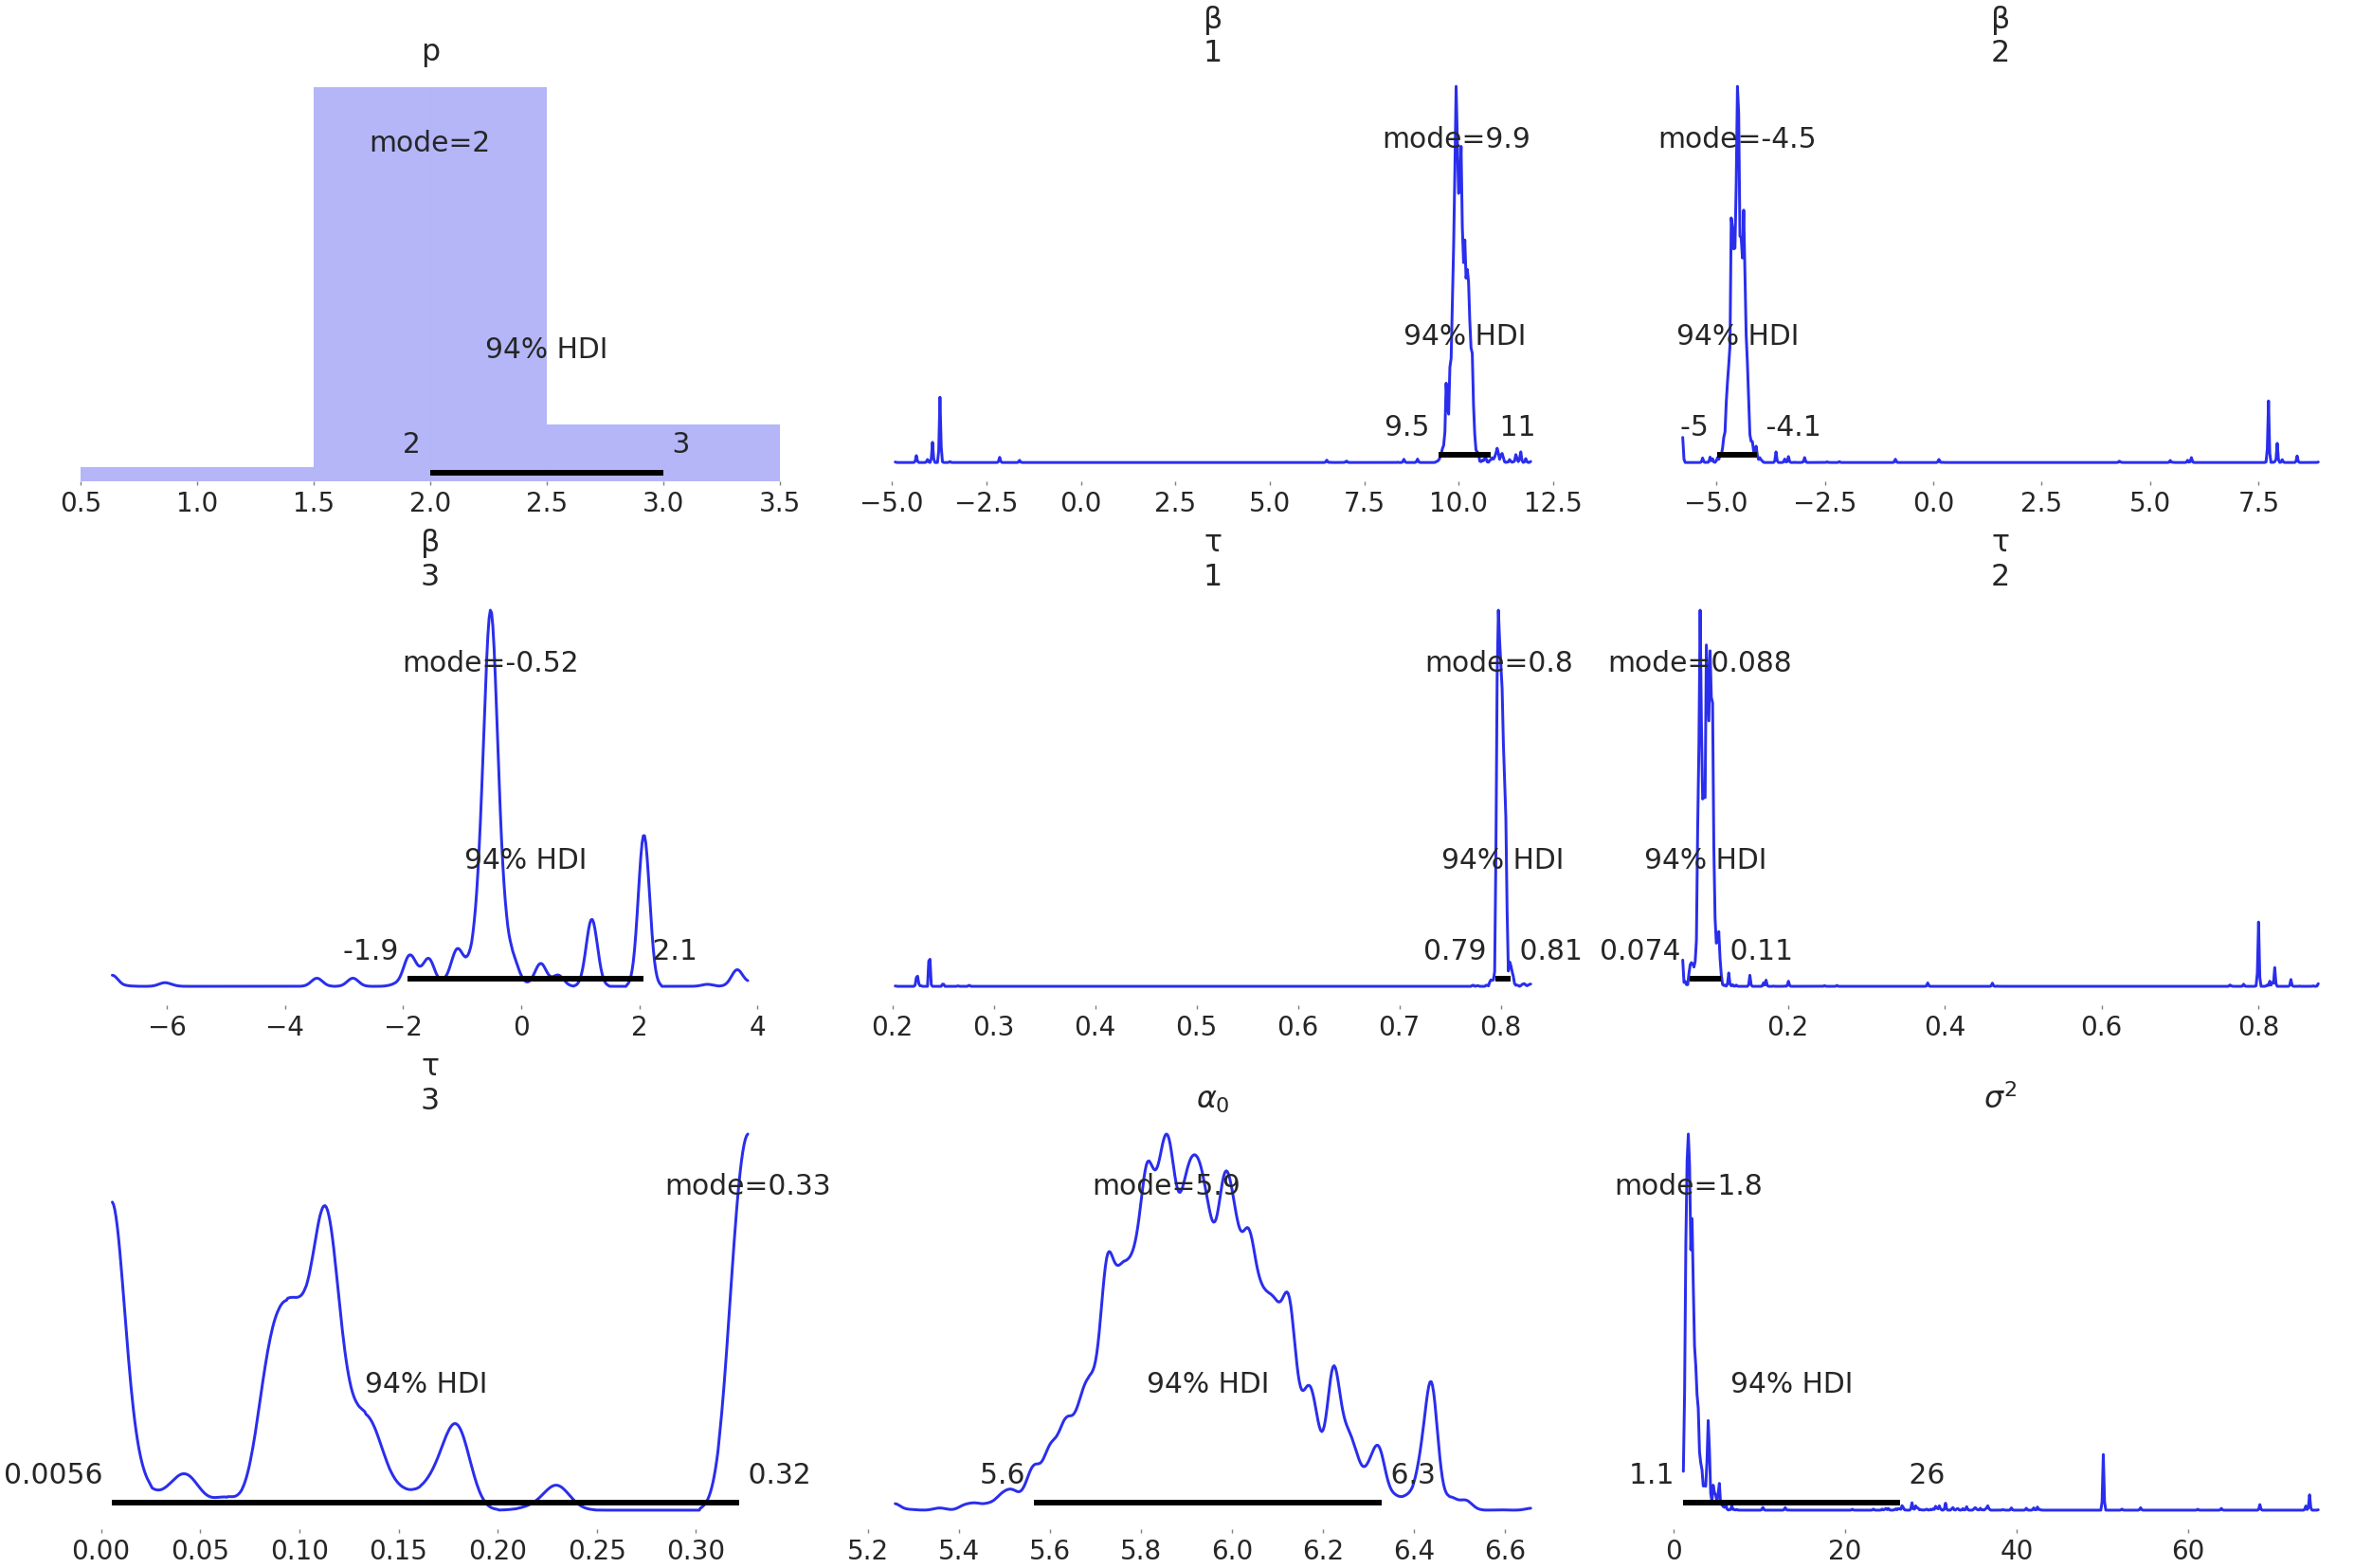
\includegraphics[width=.9\textwidth]{posterior}
  \end{figure}

Many alternatives: Metropolis-Hastings, \maroon{emcee}, Hamiltonian Monte Carlo, \ldots.
\end{frame}

\begin{frame}{Label switching}
The model suffers from non-identifiability of the components caused by their interchangeability: \(\pi(Y|X,\theta)=\pi(Y|X, \nu(\theta))\) for any permutation \(\nu\) that rearranges the indices \(j=1,\dots, p\):
    \[
    (\beta_1, \beta_2, \tau_1, \tau_2, \alpha_0, \sigma^2) \leftrightsquigarrow (\beta_2, \beta_1, \tau_2, \tau_1, \alpha_0, \sigma^2).
  \]

Hence, the components may be inadvertently exchanged from one iteration to the next in any MCMC algorithm.

\metroset{block=transparent}
\vspace{1em}
\begin{alertblock}{Partial solution}
  \vspace{0.25em}
  Post-process the trace and impose an artificial identifiability constraint on the parameters, such as \(\beta_i < \beta_j\) if \(i<j\) (or the analogous with \(\tau\)).
\end{alertblock}
\metroset{block=fill}
\end{frame}

\begin{frame}{Predictions}
  \textbf{Summarize-then-predict}. A summary of the posterior distribution \(\theta| \D_n\) is obtained via a point-estimate statistic (mean, median, mode), and then predictions are made according to the assumed model, e.g.:
  \[
  \hat Y_i =\hat \alpha_0 + \sum_{j=1}^p \hat \beta_j X_i(\hat t_j), \quad i=1,\dots, n.
  \]

  \textbf{Predict-then-summarize}. We first construct predictions on each step of the MCMC algorithm following our model, i.e.:
  \[
    Y_i^{(m)*} \equiv Y_i \mid X_i, \theta^{(m)*}, \quad m=1,\dots,M, \quad i=1,\dots, n.
  \]
  Then, the mean of all such intermediate predictions is used as a proxy for the response variable:
  \[
    \hat Y_i = \frac{1}{M}\sum_{m=1}^M Y_i^{(m)*}, \quad i=1,\dots, n.
  \]
\end{frame}

\begin{frame}{Predictions (cont.)}
    We are essentially approximating the \textit{posterior predictive distribution}
\[
\pi(y\mid x, \D_n) = \int_{\Theta} \pi(y\mid x, \theta)\pi(\theta\mid \D_n)\, d\theta.
\]
  \begin{figure}
    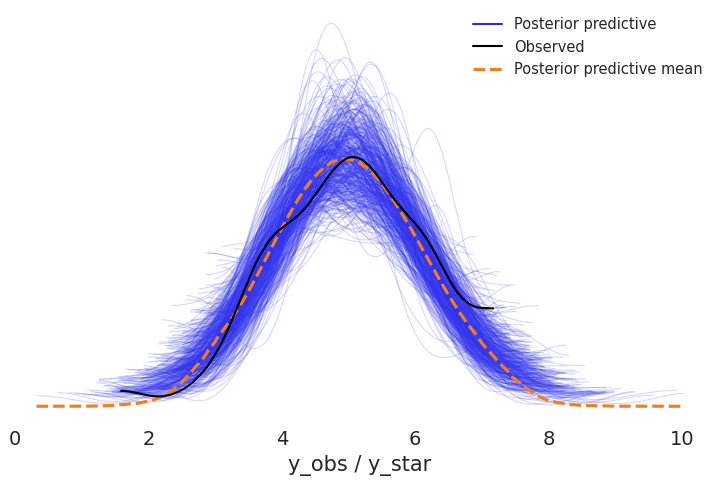
\includegraphics[width=.675\textwidth]{ppc_linear}
  \end{figure}
\end{frame}

\begin{frame}{Predictions (cont.)}
    \textbf{Variable selection}. We select \(p\) variables using only a point estimator of \(\tau|\D_n\) (so-called \textit{impact points}), and then we can apply any multiple regression algorithm to the reduced data set.
    \vspace{1em}

    \begin{figure}
      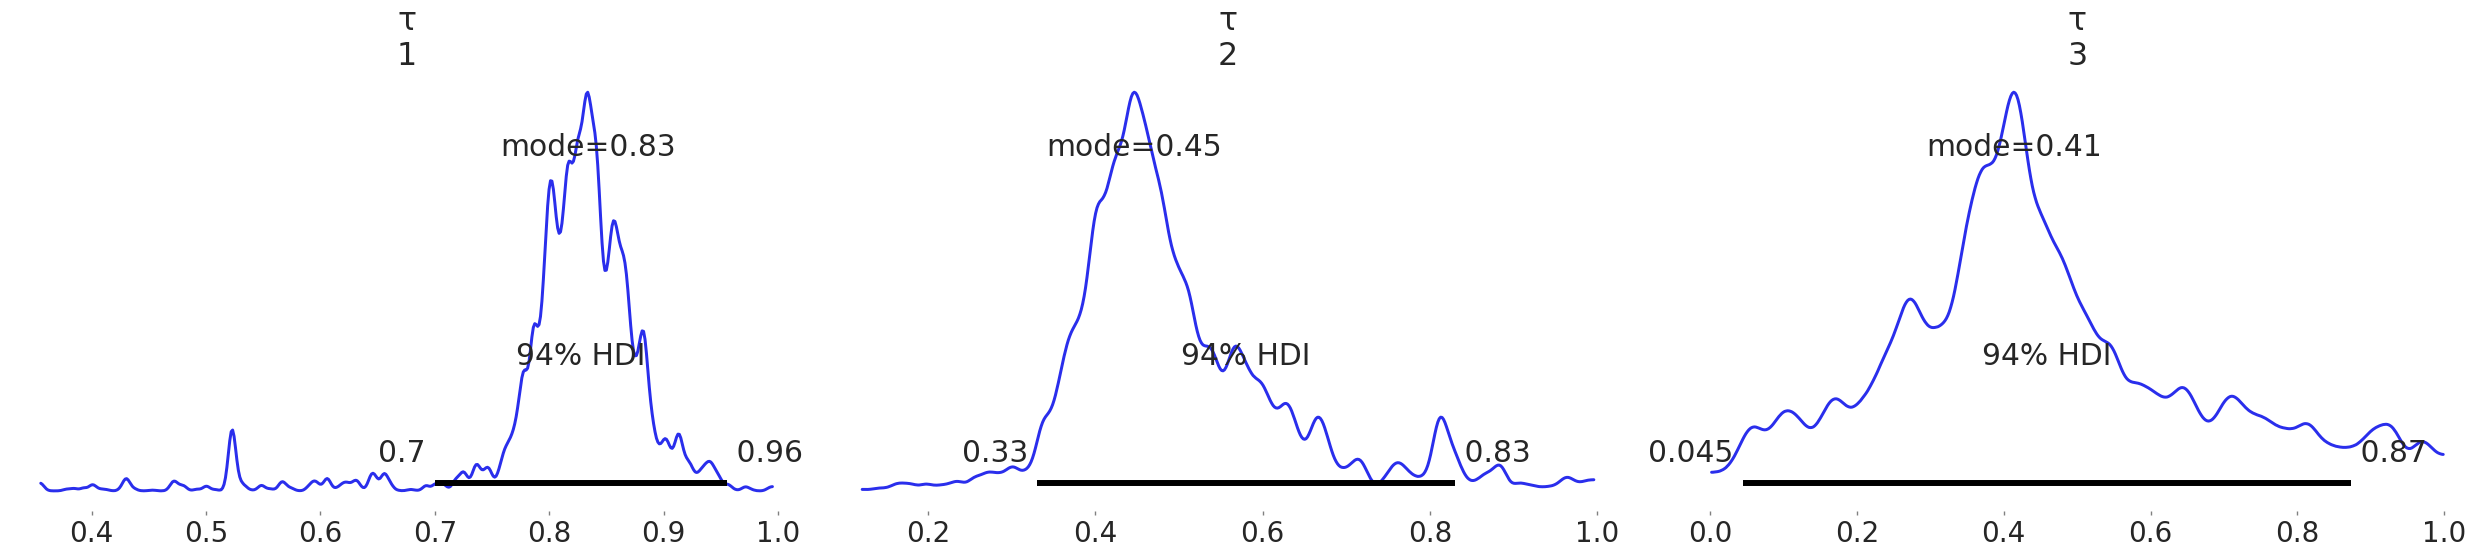
\includegraphics[width=\textwidth]{credible_intervals}
    \end{figure}

    At any rate, all the above predictors can be obtained after a single run of the MCMC algorithm.
\end{frame}

\section{Experiments}

\begin{frame}{Methodology}
  \begin{itemize}
    \item Experiments on simulated data, with \(250\) samples of different Gaussian and non-Gaussian processes on a regular grid of \(100\) points. Also experiments on real data sets.
    \item We perform 10 random train/test partitions (60\%/40\%) to account for the stochasticity of the model, along with \(5\)-fold cross-validation to select the best hyperparameters on the training set.
    \item The hyperparameters of our models are \(p\in\{1,2,\dots,10\}\), \(g=5\) and \(\eta \in \{10^{-4}, 10^{-3}, \dots, 10^2\}\).
    \item Several regression methods are considered for comparison, along with variable selection techniques, functional or otherwise. The evaluation metrics are the RMSE and the accuracy.
  \end{itemize}
\end{frame}

\begin{frame}{Linear regression: simulated GP-RKHS data}
  \[
  Y=5 -5X(0.1) + X(0.4) + 10X(0.8) + \epsilon, \quad \epsilon \sim \mathcal N(0, 0.5).
  \]
  \begin{figure}
    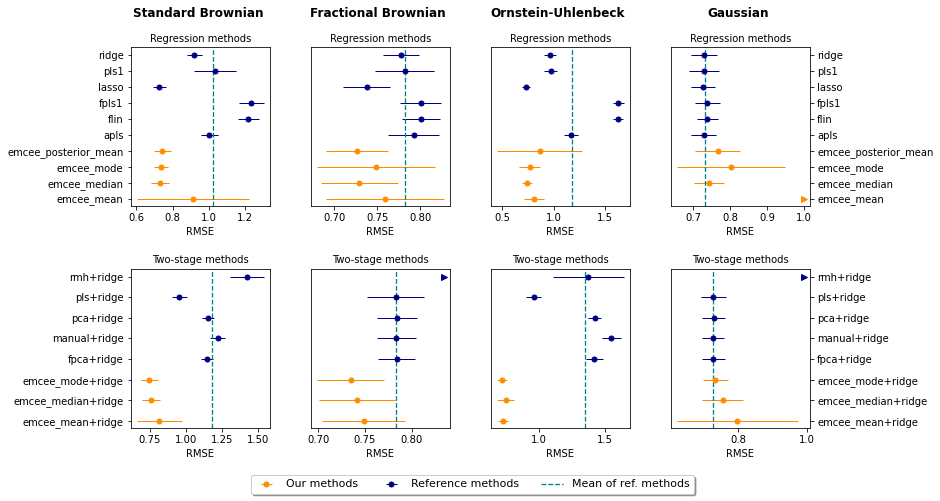
\includegraphics[width=.95\textwidth]{reg_emcee_rkhs}
  \end{figure}
\end{frame}

\begin{frame}{Linear regression: simulated GP-\(\bm{L^2}\) data}
  \[
  Y = 5 + \int_0^1 \log(1+4t)X(t)\, dt + \epsilon, \quad \epsilon \sim \mathcal N(0, 0.5).
  \]
  \begin{figure}
    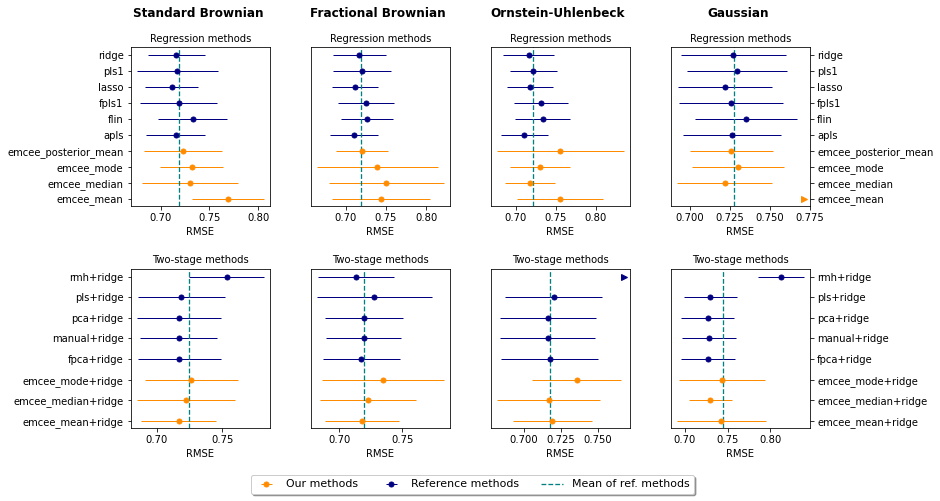
\includegraphics[width=.95\textwidth]{reg_emcee_l2}
  \end{figure}
\end{frame}

\begin{frame}{Linear regression: simulated non-GP data}
  \[
  X(t) = e^{BM(t)}, \quad BM \equiv \text{standard Brownian motion}.
  \]
  \begin{figure}
    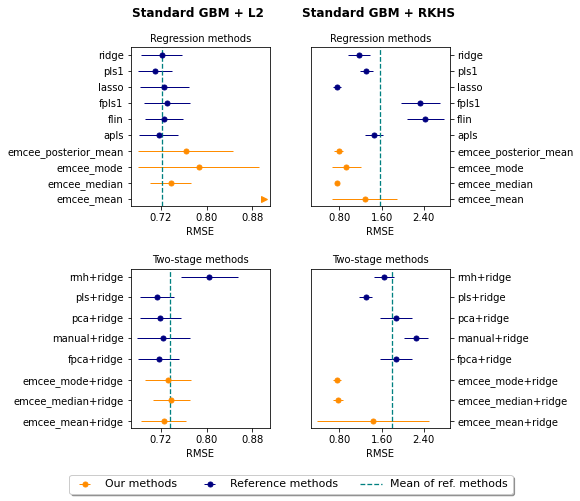
\includegraphics[width=.6\textwidth]{reg_emcee_nongp}
  \end{figure}
\end{frame}

\begin{frame}{Linear regression: real data}
  \begin{center}
    Three real data sets.
  \end{center}
    \vspace{.5em}
  \begin{figure}
    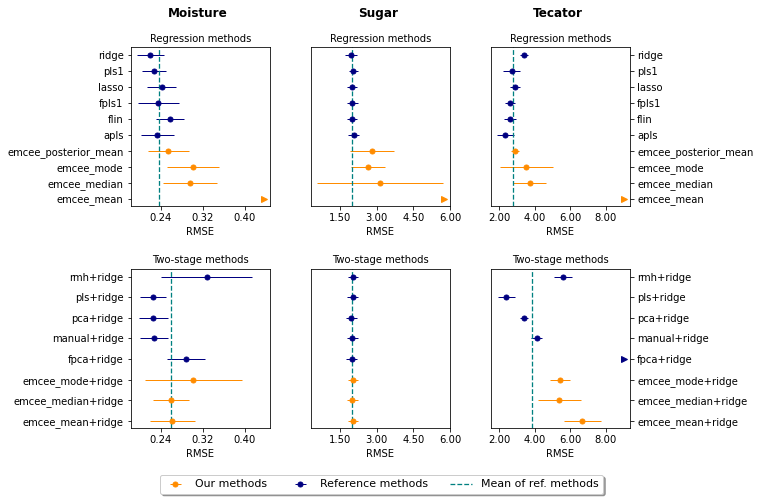
\includegraphics[width=.8\textwidth]{reg_emcee_real}
  \end{figure}
\end{frame}

\begin{frame}{Logistic regression: simulated GP-RKHS data}
\[
  \P(Y=1\mid X) = \frac{1}{1 + \exp\left\{0.5 +5X(0.1) - X(0.4) - 10X(0.8)\right\}}.
\]
  \begin{figure}
    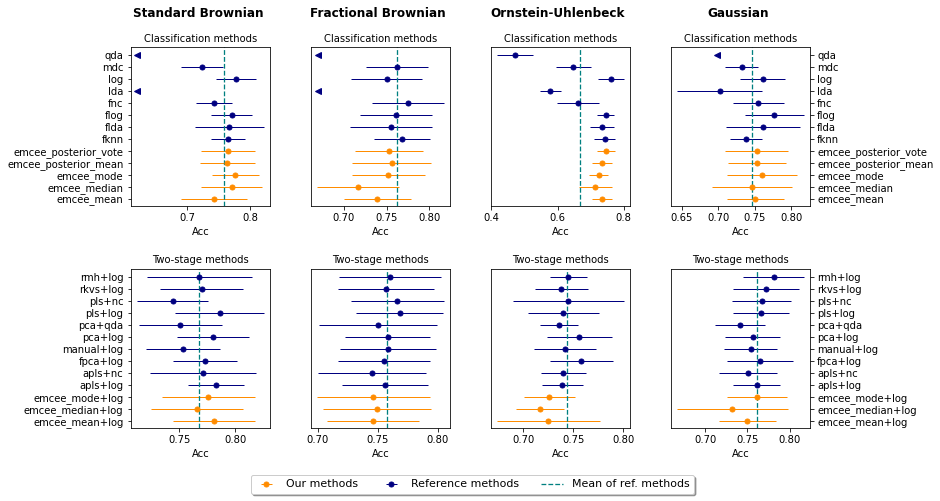
\includegraphics[width=.95\textwidth]{clf_emcee_rkhs}
  \end{figure}
\end{frame}

\begin{frame}{Logistic regression: simulated GP-\(\bm{L^2}\) data}
  \[
  \P(Y=1\mid X) = \frac{1}{\displaystyle 1 + \exp\left\{0.5 - \int_0^1 \log(1+4t) X(t)\, dt\right\}}.
  \]
  \begin{figure}
    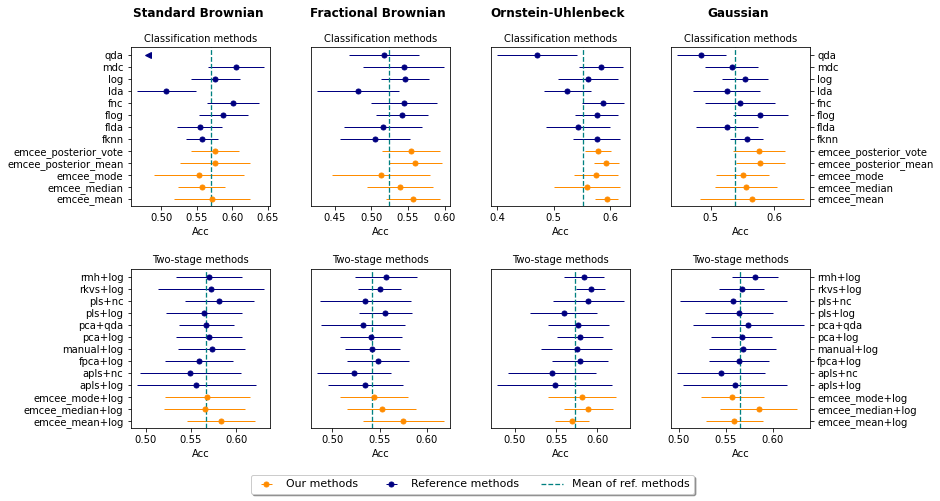
\includegraphics[width=.95\textwidth]{clf_emcee_l2}
  \end{figure}
\end{frame}

\begin{frame}{Logistic regression: simulated non-GP data}
  \[
  X^{\text{hom}} \sim BM(0, 1) + BM(m(t), 1), \quad X^{\text{het}} \sim BM(0, 1) + BM(0, 2).
  \]
  \begin{figure}
    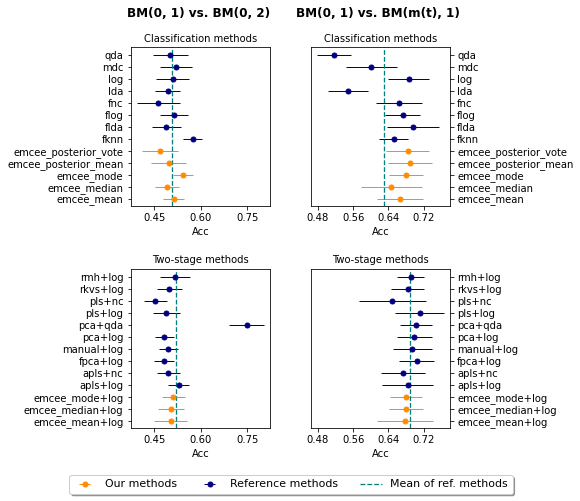
\includegraphics[width=.6\textwidth]{clf_emcee_nongp}
  \end{figure}
\end{frame}

\begin{frame}{Logistic regression: real data}
  \begin{center}
    Three real data sets.
  \end{center}
    \vspace{.5em}
  \begin{figure}
    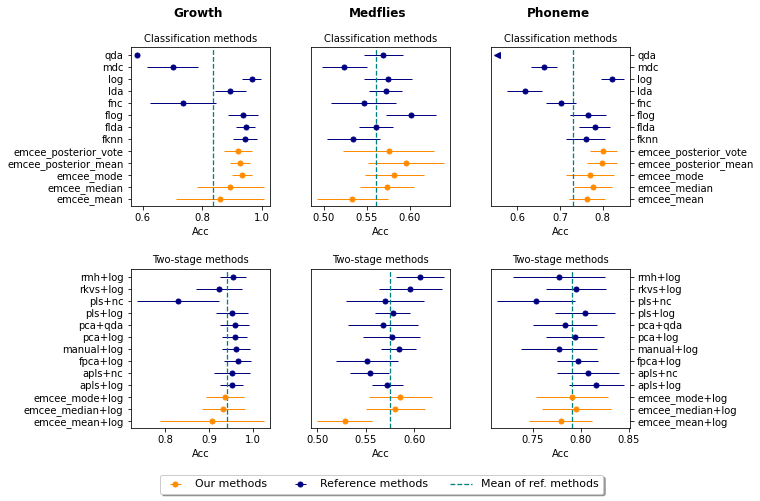
\includegraphics[width=.8\textwidth]{clf_emcee_real}
  \end{figure}
\end{frame}

\begin{frame}{Other experiments}
\begin{itemize}
  \item Recover the underlying data generation model when it is a finite-dimensional RKHS model.
  \item Incorporate \(p\) into the Bayesian scheme with a categorical distribution.
  \item Change some prior distributions, such as Cauchy for \(\sigma^2\) or Beta for the times \(\{t_j\}\).
  \item Try different ways to address the label switching problem.
\end{itemize}
\end{frame}

\section{Conclusions}

\begin{frame}{Conclusions and future work}

     \metroset{block=transparent}
 \begin{alertblock}{Our proposal}
   \begin{itemize}
     \item Simple and interpretable finite-dimensional approximation to functional regression.
     \item Computationally feasible Bayesian approach to parameter estimation within the proposed model.
     \item Python implementation competitive with usual alternatives in both simulated and real data sets.
   \end{itemize}
 \end{alertblock}

\pause

 \begin{exampleblock}{The road ahead}
   \begin{itemize}
     \item Experiment with different prior distributions.
     \item Derive theoretical properties of the predictors.
     \item Try different MCMC algorithms (e.g. reversible-jump MCMC).
   \end{itemize}
 \end{exampleblock}

\end{frame}

\begin{frame}
    \frametitle{References}
    \nocite{*}
    \printbibliography[heading=none]
\end{frame}

\appendix

\begin{frame}[standout]
  Thank you for your attention
\end{frame}



%%
% BACKUP SLIDES
%%

\begin{frame}{Dependence on \(\bm p\)}
Mean accuracy for our logistic RKHS methods as a function of \(p\), using \(\eta=0.01\) and the homoscedastic mixture data set.

\vspace{1em}

\begin{figure}
  \centering
  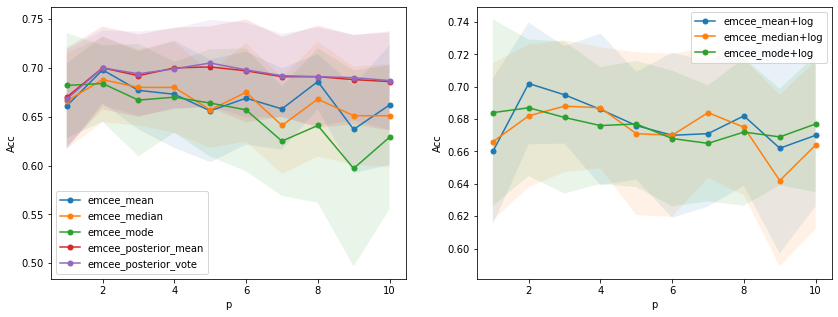
\includegraphics[width=.95\textwidth]{mixture_dependence_acc_p}
  \caption*{}
\end{figure}
\end{frame}

\begin{frame}{Recovering the underlying model}
  \vspace{1em}
  Underlying finite-dimensional RKHS data generation model with 2 components.

  \vspace{.5em}
\begin{figure}[b]

  \begin{subfigure}[b]{0.48\textwidth}
    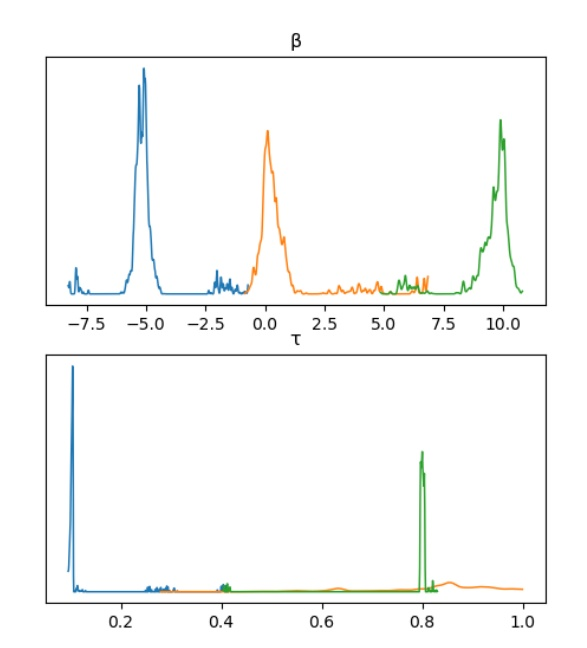
\includegraphics[width=.95\textwidth]{beta_3}
    \caption{RKHS model with \(p=3\).}
  \end{subfigure}
  \hfill
  \begin{subfigure}[b]{0.48\textwidth}
    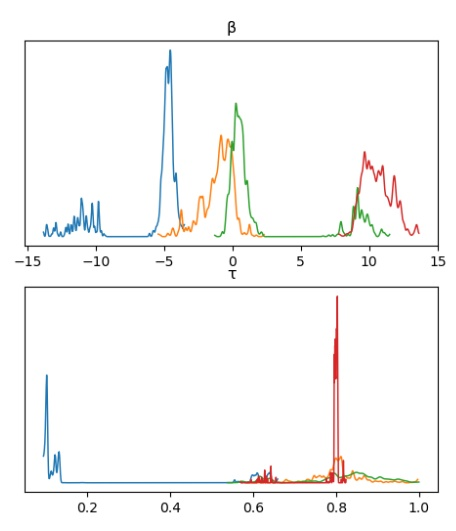
\includegraphics[width=.9\textwidth]{beta_4}
    \caption{RKHS model with \(p=4\).}
  \end{subfigure}
\end{figure}
\end{frame}

\begin{frame}{Metropolis-Hastings}
  Approximate a distribution \(\pi(x)\) such that \(\pi(x)\propto f(x)\):
  \begin{enumerate}
  \item Generate a proposal \(x' \sim g(x'|x_t)\).
  \item Accept the proposal with probability \(\alpha=\min\{1, f(x')/f(x_t)\}\). If accepted, set \(x_{t+1}=x'\); otherwise set \(x_{t+1}=x_t\).
\end{enumerate}

\vspace{1em}

 \begin{figure}
   \centering
   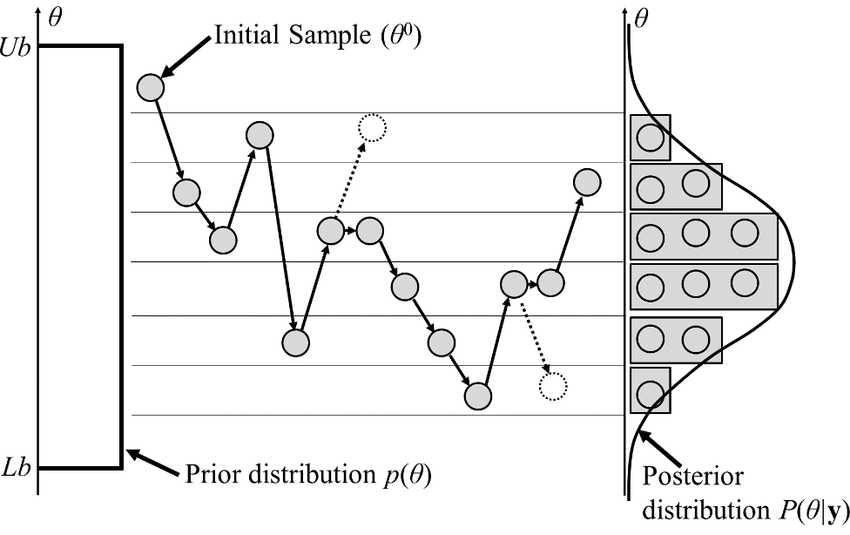
\includegraphics[width=.6\textwidth]{mh}
 \end{figure}
\end{frame}

\begin{frame}{Affine-invariant ensemble sampler (emcee)}
Consider an \maroon{ensemble} \ of walkers \(\Lambda(t) = (\Lambda_1(t), \dots, \Lambda_L(t))\) and the complementary ensemble
\[
  \Lambda_{-l}(t) = \{\Lambda_1(t+1), \dots, \Lambda_{l-1}(t+1), \Lambda_{l+1}(t), \dots, \Lambda_L(t)\}, \quad l=1,\dots, L.
\]
\vspace{-1em}
\begin{enumerate}
  \item For each walker \(1\leq l \leq L\) another walker \(\Lambda_j \in \Lambda_{-l}(t)\) is chosen at random. The proposal is constructed as
  \[
    \Lambda_l(t) \to \Gamma = \Lambda_j + Z(\Lambda_l(t) - \Lambda_j),
\]
where \(Z \stackrel{i.i.d.}{\sim} g(z)\) satisfying \(g(z^{-1})=zg(z)\).

\item If \(\R^p\) is the sample space, the proposal is accepted with probability
  \[
    \alpha = \min\left\{1, \ Z^{p-1}\frac{\pi(\Gamma)}{\pi(\Lambda_l(t))}\right\}.
  \]
\end{enumerate}
\end{frame}

\end{document}
